\subsection{Recolectar los datos Iniciales}
    Los datos utilizados durante el transcurso del proyecto fueron obtenidos
    gratuitamente en el sitio de Kaggle y el mismo se encuentra en formato csv.
    \subsubsection{Reporte de la recolección de datos iniciales}
        \begin{itemize}
            \item El data set se encuentra en la carpeta ```src/data/``` del proyecto.
            \item Se uso pandas como metodo de recoleccion de datos.
            \item Para poder levantar el set de datos se usa como separado una coma.
        \end{itemize}
\subsection{Descubrir datos}
    \subsubsection{Reporte de descripción de datos}
        Se cuenta con dos datasets: por un lado se tienen datos estadísticos y
        generales de los videos descritos en 16 columnas; por otro lado hay un
        archivo json con el nombre de cada categoria segun el numero asignado.
        A continuación, los nombres de los features con su correspondiente
        descripción y tipo de dato:
        \resizebox{\columnwidth}{!}{\begin{tabular}{||c | c | c||}
            \hline
            \textbf{Mombre de variable} & \textbf{tipo de dato} & \textbf{Descripcion} \\ [0.5ex]
            \hline\hline
            video\_id & alfanumerica & identifica a cada video \\
            \hline
            trending\_date & date & Es una fecha en un dia especifico luego de la publicacion del video \\
            \hline
            title & alfanumerica & Es el titulo del video \\
            \hline
            channel\_title & alfanumerica & Es el nombre del canal del usuario que publico el videoo \\
            \hline
            category\_id & numeric & it is the number that represent a category nameo \\
            \hline
            publish\_time & timestamp & momento exacto de la publicacion del videoo \\
            \hline
            tags & alfanumerico & Etiquetas que se pueden agregar al videoo \\
            \hline
            views & numeric & Cantidad de vistas del video en el momento de la fecha de trending\_dateo \\
            \hline
            likes & numeric & Cantidad de me gusta que el video tiene dados por usuarios de la plataforma youtubeo \\
            \hline
            dislikes & numeric & Cantidad de no me gusta que el video tiene dados por usuarios de la plataforma youtubeo \\
            \hline
            comment\_count & numeric & Cantidad de comentarios del videoo \\
            \hline
            thumbnail\_link & url & enlace ao \\
            \hline
            comments\_disabled & booleano & Dice si tiene o no los comentarios habilitadoso \\
            \hline
            ratings\_disabled & booleano & Dice si tiene o no los likes/dislikes habilitadoso \\
            \hline\
            video\_error\_or\_removed & booleano & Dice si el video sufrio un error o fue borrado en el momento de la fecha de trending\_dateo \\
            \hline
            description & alfanumeric & Texto escrito por el creador del video que describe el mismoo \\
            \hline
        \end{tabular}}
\newpage
\subsection{Exploración de los datos}
    \subsubsection{Reporte de exploración de datos}

            \paragraph{Analisis de categorias}
                \begin{figure}[ht]
                    \begin{adjustbox}{addcode={
                        \begin{minipage}{\width}}{
                            \caption{%
                                Cantidad de videos segun la categoria
                                }
                        \end{minipage}},rotate=360,center}
                        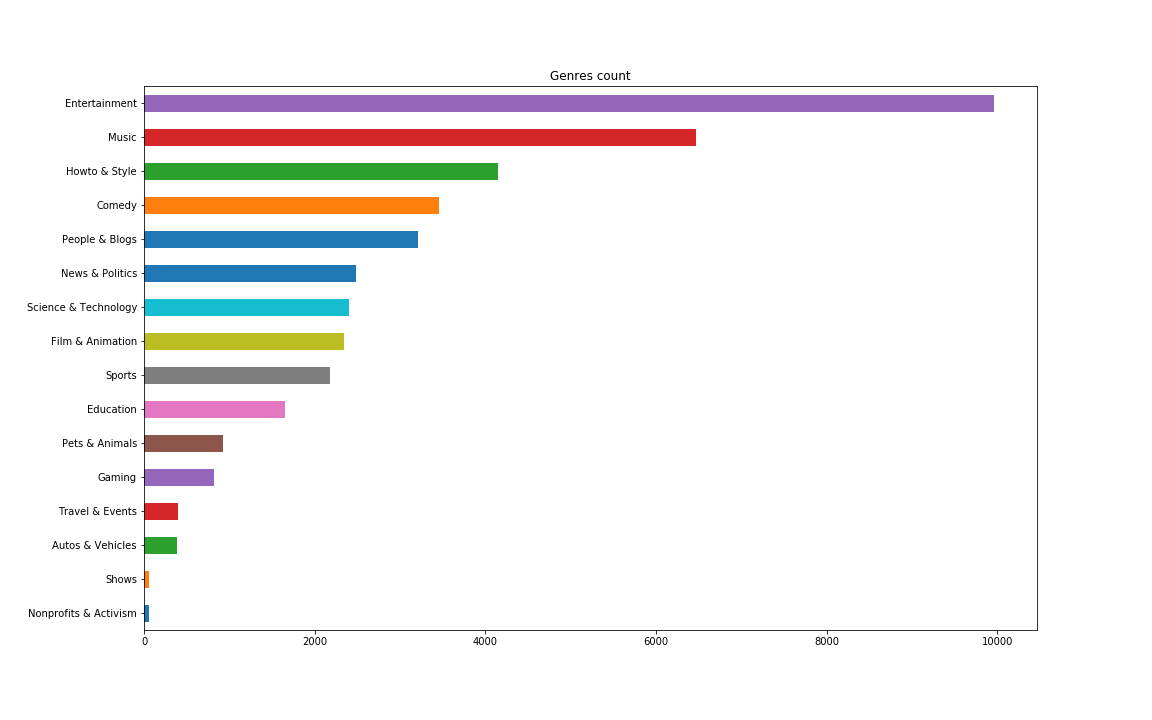
\includegraphics[scale=.5]{../doc/report/pics/Analisis-de-categorias.png}
                    \end{adjustbox}
                \end{figure}
            \FloatBarrier

        \newpage
        \paragraph{Analisis de vistas en funcion de likes}

            \begin{figure}
                \begin{adjustbox}{addcode={
                    \begin{minipage}{\width}}{
                        \caption{%
                            Cantidad de vistas segun la cantidad de likes
                            }
                    \end{minipage}},rotate=360,center}
                    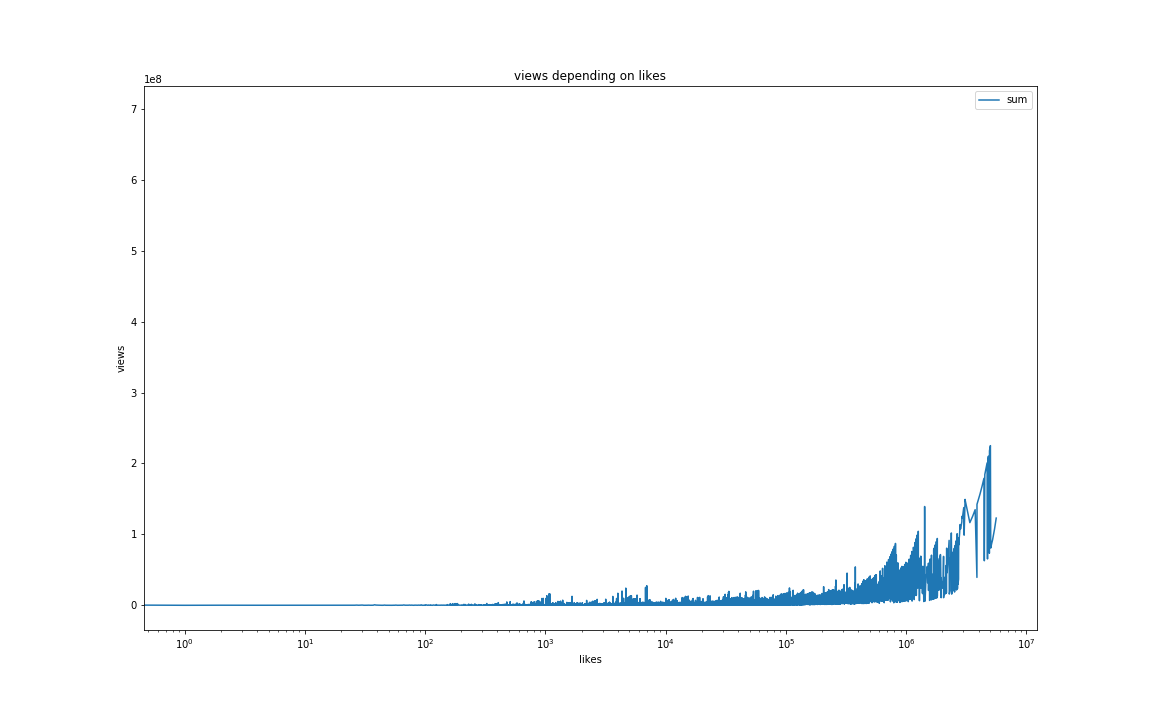
\includegraphics[scale=.6]{../doc/report/pics/Analisis_de_vistas_en_funcion_de_likes.png}
                \end{adjustbox}
            \end{figure}
        \FloatBarrier
        Podemos observar que hay un punto de quiebre en el cual a partir de
        cierta cantidad de likes los videos tienden a aumentar su cantidad
        de vistas

        \newpage
        \paragraph{Analisis de vistas en funcion de la diferencia de dias entre la fecha de tendencia y la de publicacion}

            \begin{figure}[ht]
                \begin{adjustbox}{addcode={
                    \begin{minipage}{\width}}{
                        \caption{%
                            Cantidad de vistas a medida que pasan los dias de su publicacion
                            }
                    \end{minipage}},rotate=360,center}
                    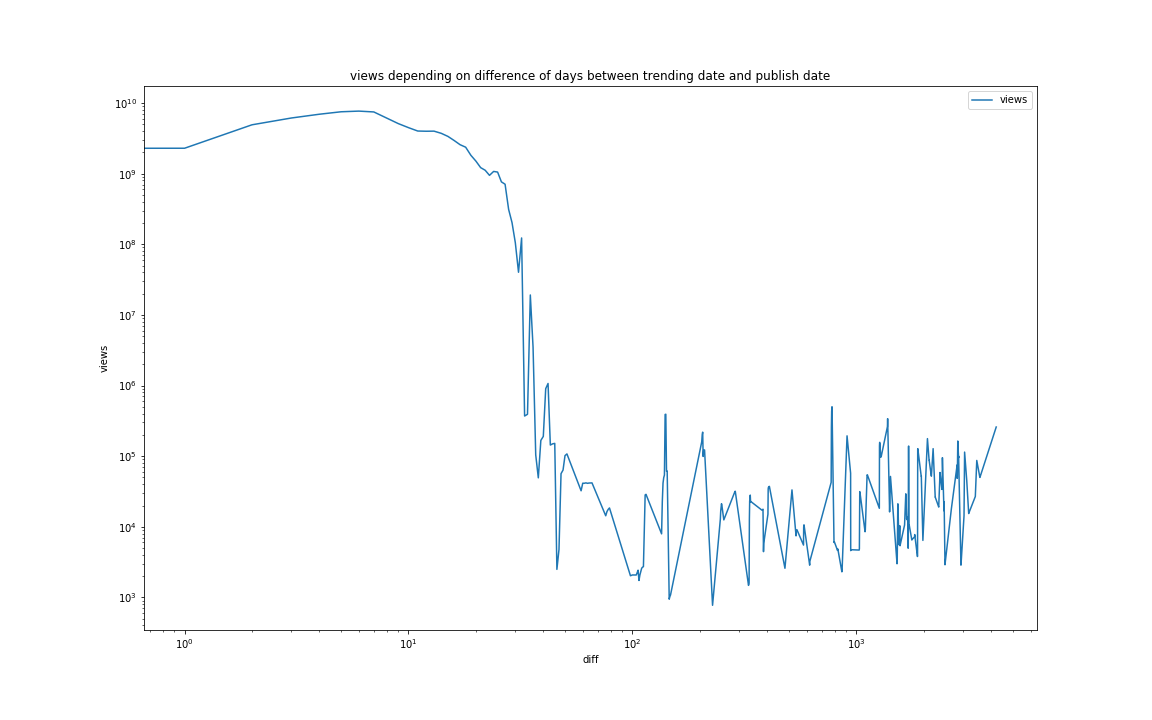
\includegraphics[scale=.6]{../doc/report/pics/Analisis_de_vistas_en_funcion_de_la_diferencia_de_dias_entre_la_fecha_de_tendencia_y_la_de_publicacion.png}
                \end{adjustbox}
            \end{figure}
        \FloatBarrier
        Podemos observar que el mayor incremento en la cantidad de vistas es a
        los pocos dias de la fecha de publicacion del video. Luego vemos que
        las vistan tienden a decaer

        \newpage
        \paragraph{Analisis de vistas en funcion de la diferencia de likes y dislikes}

            \begin{figure}[ht]
                \begin{adjustbox}{addcode={
                    \begin{minipage}{\width}}{
                        \caption{%
                            Cantidad de vistas segun la diferencia entre likes y dislikes
                            }
                    \end{minipage}},rotate=360,center}
                    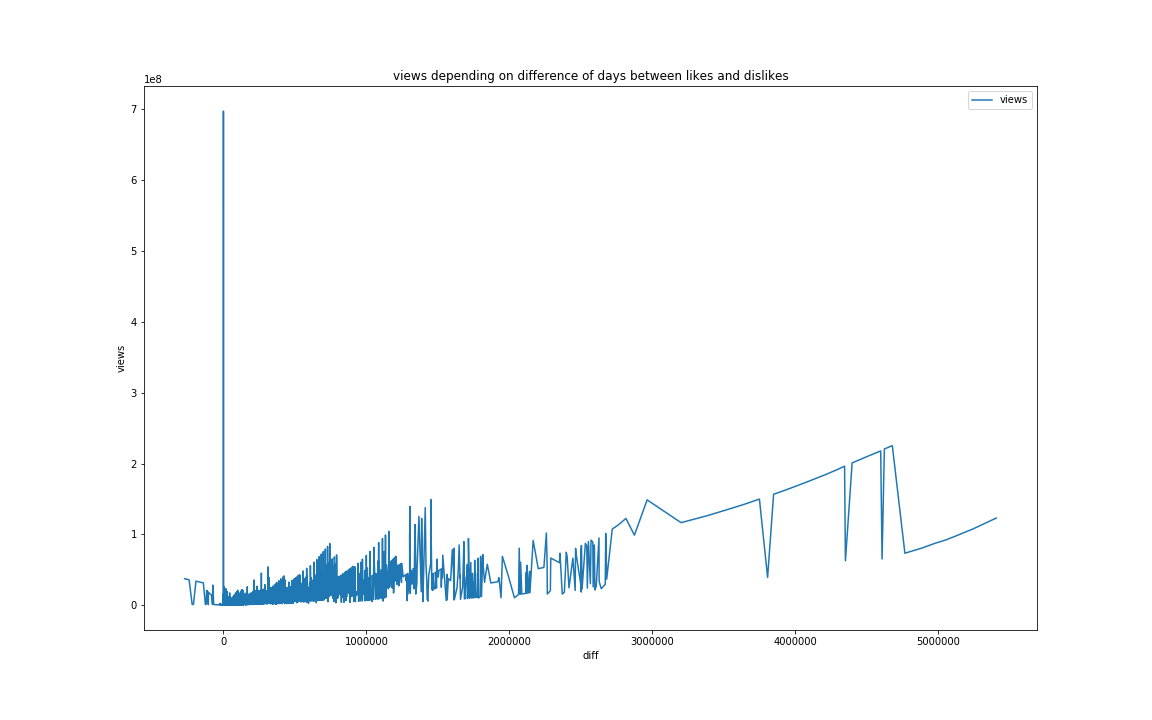
\includegraphics[scale=.6]{../doc/report/pics/Analisis_de_vistas_en_funcion_de_la_diferencia_de_likes_y_dilikes.png}
                \end{adjustbox}
            \end{figure}
        \FloatBarrier
        Podemos observar a medida que aumenta la distancia entre likes y dislikes,
        aumentan la cantidad de vistas. Esto es logico ya que en general un video
        tiene mas vistas cuanto mas gente descata que el mismo le gusto.

        \newpage
        \paragraph{Analisis del progreso de views del video con mayor views del set de datos.}

            \begin{figure}[ht]
                \begin{adjustbox}{addcode={
                    \begin{minipage}{\width}}{
                        \caption{%
                            Progreso en dias de las vistas del video mas vistas
                            }
                    \end{minipage}},rotate=360,center}
                    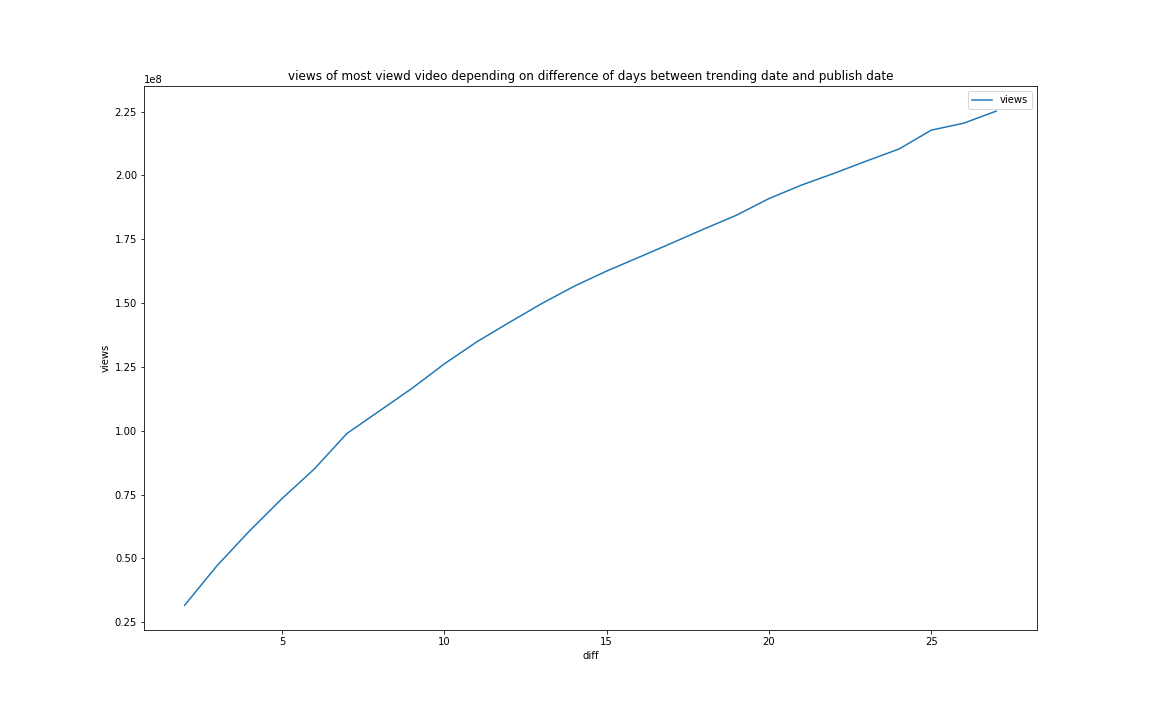
\includegraphics[scale=.6]{../doc/report/pics/Analisis_del_progreso_de_views_del_video_con_mayor_views_del_set_de_datos.png}
                \end{adjustbox}
            \end{figure}
        \FloatBarrier
        Podemos observar que a medida que pasan los dias respecto de la fecha de
        publicacion del video con mas vistas del set de datos, las vistas del
        mismo suben linealmente, lo cual tiene sentido ya que cuando un video
        es exitoso, sus vistan tienen a aumentar progresivamente.

        \newpage
        \paragraph{Analisis del progreso de views de los videos con mayor, mediano y menor vistas del set de datos.}

            \begin{figure}[ht]
                \begin{adjustbox}{addcode={
                    \begin{minipage}{\width}}{
                        \caption{%
                            Progreso en dias de las vistas del video mas, mediano y menos vistas
                            }
                    \end{minipage}},rotate=360,center}
                    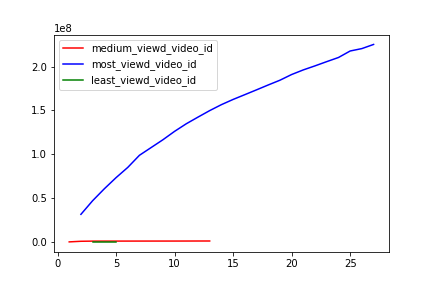
\includegraphics[scale=.6]{../doc/report/pics/Analisis_del_progreso_de_views_de_los_videos_con_mayor_mediano_y_menor_vistas_del_set_de_datos.png}
                \end{adjustbox}
            \end{figure}
        \FloatBarrier
        Podemos observar que el video menos visto y el video cuya cantidad de
        vistas es la mediana del set de datos tienen un progreso de variacion de
        vistas en el tiempo parecido. Y el video mas visto muestra una amplia
        diferencia. Esto tiene sentido ya que para tener un progreso como el que
        tiene el video mas visto se tiene que tener ciertas caracteristicas
        parecidas. Esto nos dice que hay un grupo pequeño cercano al video mas
        visto que logra este progreso. y el resto se parece al menos visto

        \newpage
        \paragraph{Analisis de la cantidad de views segun el largo del titulo del video.}

            \begin{figure}[ht]
                \begin{adjustbox}{addcode={
                    \begin{minipage}{\width}}{
                        \caption{%
                            Cantidad de vistas segun el largo del video
                            }
                    \end{minipage}},rotate=360,center}
                    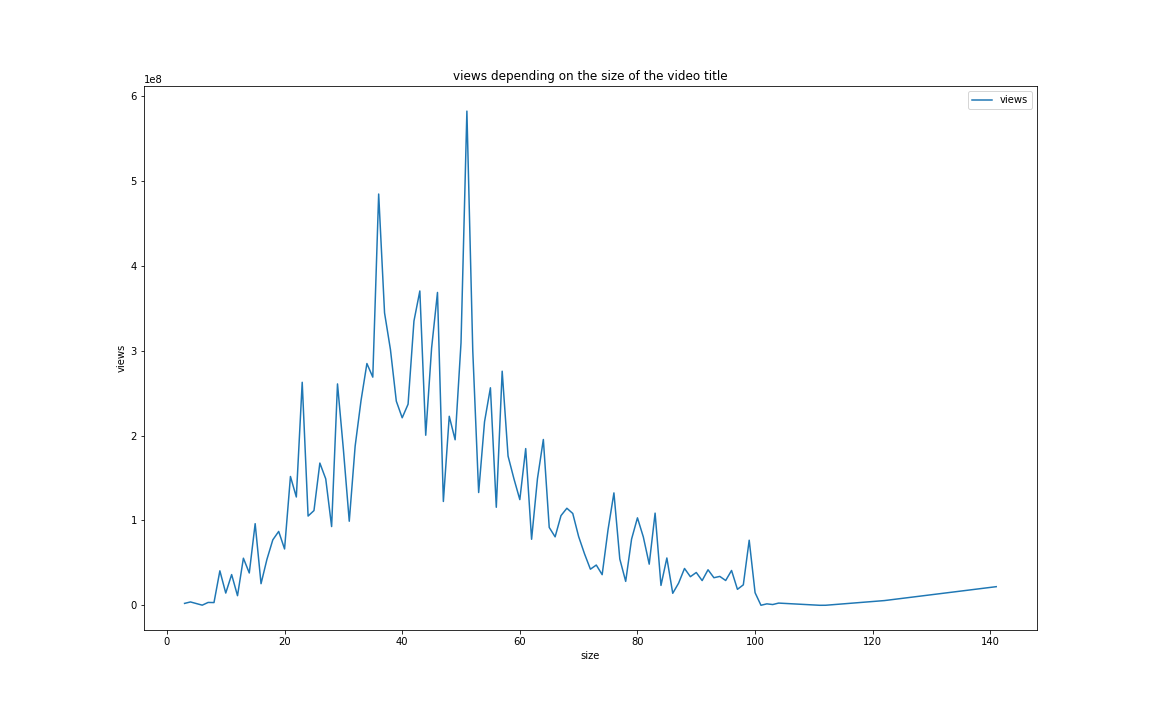
\includegraphics[scale=.6]{../doc/report/pics/Analisis_de_la_cantidad_de_views_segun_el_largo_del_titulo_del_video.png}
                \end{adjustbox}
            \end{figure}
        \FloatBarrier
        Podemos observar que el largo del titulo tiene un rango de valores para
        su largo en el cual la cantidad de vistas del video logra un valor maximo.
        Esto tiene sentido ya que el ser humano tiende a leer cosas cortas que
        generen impacto y es por eso que este rango esta cercano al cero. Tambien
        si el titulo es muy corto es logico que las vistas no sean altas ya que quizas
        signifique que ese titulo corto no describe con impacto el video y por lo tanto
        no genera una atraccion para que la gente lo mire.

        \newpage
        \paragraph{Analisis la cantidad de videos borrados por categoria.}

            \begin{figure}[ht]
                \begin{adjustbox}{addcode={
                    \begin{minipage}{\width}}{
                        \caption{%
                            Cantidad de videos borrados por cateogria
                            }
                    \end{minipage}},rotate=360,center}
                    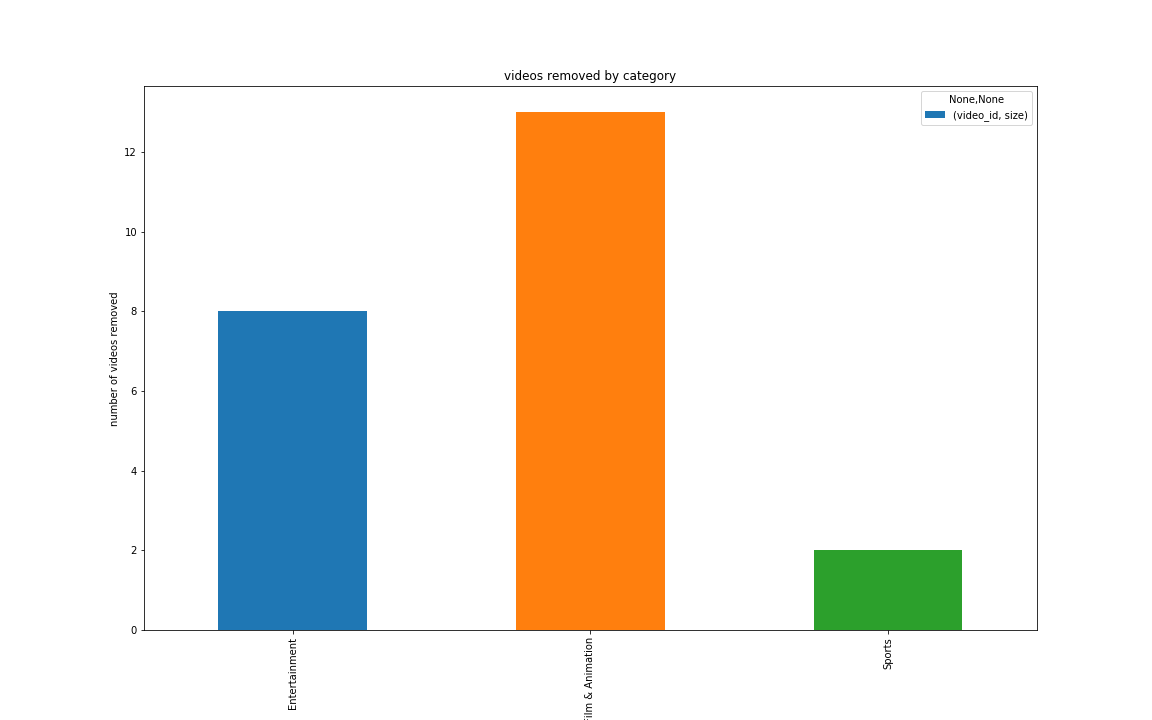
\includegraphics[scale=.6]{../doc/report/pics/Analisis_la_cantidad_de_videos_borrados_por_categoria.png}
                \end{adjustbox}
            \end{figure}
        \FloatBarrier
        Podemos observar que solo en las categorias entretenimeinto, deportes y
        animacion hay videos que fueron borrados. Esto es probable que se deba a
        problemas de copywright ya que youtube tiene ciertas resctricciones cuando
        se muestran imagenes que pertenecen a otras marcas, canciones o peliculas.
        Youtube ofrece un tiempo maximo para poner una cancion ajena hasta que te
        bloquean o desmonetizan el video por copywright. Lo mismo ocure con peliculas,
        o deportes.

        \newpage
        \paragraph{Analisis de la cantidad de vistas de videos segun tenga o no descripcion.}

            \begin{figure}[ht]
                \begin{adjustbox}{addcode={
                    \begin{minipage}{\width}}{
                        \caption{%
                            Cantidad de vistas segun su descripcion este o no habilitada
                            }
                    \end{minipage}},rotate=360,center}
                    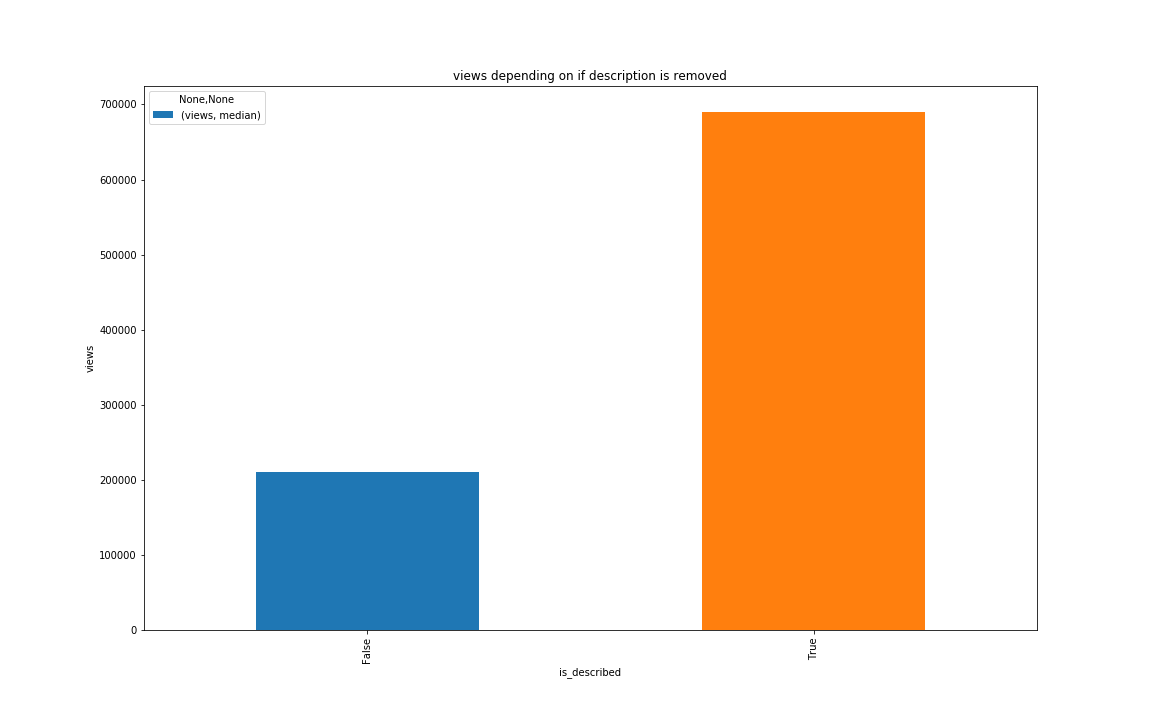
\includegraphics[scale=.6]{../doc/report/pics/Analisis_de_la_cantidad_de_vistas_de_videos_segun_tenga_o_no_descripcion.png}
                \end{adjustbox}
            \end{figure}
        \FloatBarrier
        Podemos observar que hay una mayor cantidad de videos con vistas altas
        en la mediana lo cuales cuentan con una descrpicion. Y los videos que
        no tiene descrippcion en general tienden a tener pocas vistas. Esto es
        probable que se deba a que cuando uno ve una lista de videos en yotube,
        se tiene una vista previa del mismo, se lee el titulo y un poco la
        descripcion. Esto es importante a la hora de decidir si uno le interesa
        ver ese video o no ya que te puede brindar una explicacion que te
        interese.

\subsection{Verificación de calidad de datos}
    \subsubsection{Reporte de calidad de datos}
        Los datos utilizados durante el transcurso del proyecto fueron obtenidos
        gratuitamente en el sitio de Kaggle y el mismo se encuentra en formato csv.
        Con millones de aplicaciones en la actualidad, el conjunto de datos se
        ha convertido en la clave para obtener las mejores los mejores videos
        que se publicaron en youtube. Este conjunto de datos contiene más de
        40000 detalles de videos publicados en youtube.\\\\
        Fecha de recolección de datos (de API): Abril 2019
